\section{Timing Considerations}
To assign correct neutron energies, the time resolution of the time-of-flight
detector is critical. Several tests and corrections were applied to improve
timing resolution as much as possible.

The DT5730 provides leading-edge discrimination (LED) and constant-fraction discrimination
(CFD) modes for timing determination. In pre-experiment testing, we found that using the
on-board CFD calculation increased the time required to process each event by 40
ns or more, an unacceptable increase in the per-event deadtime. Thus we chose
to use the digitizer's faster LED option and to calculate precise event timing
in software, after the experiment, by analyzing the digitized waveform for each event.
Data taken from the left and right detectors separately and gated by neutron energy 
is shown in Figs. \ref{LRCorrelation} and \ref{LRTimeDifferenceByEnergy}. 
For each energy range, the FWHM of the distribution was calculated and a hyperbolic fit was
performed, shown in Fig. \ref{DifferenceThresholdsFit}. The inherent left-right timing 
resolution, independent of neutron energy, was identified as 0.34 ns FWHM.
When folded over the actual beam energy profile (as during the experiment)
the left-right time resolution dropped to 0.52 ns.

\begin{figure}[h]
    \centering
    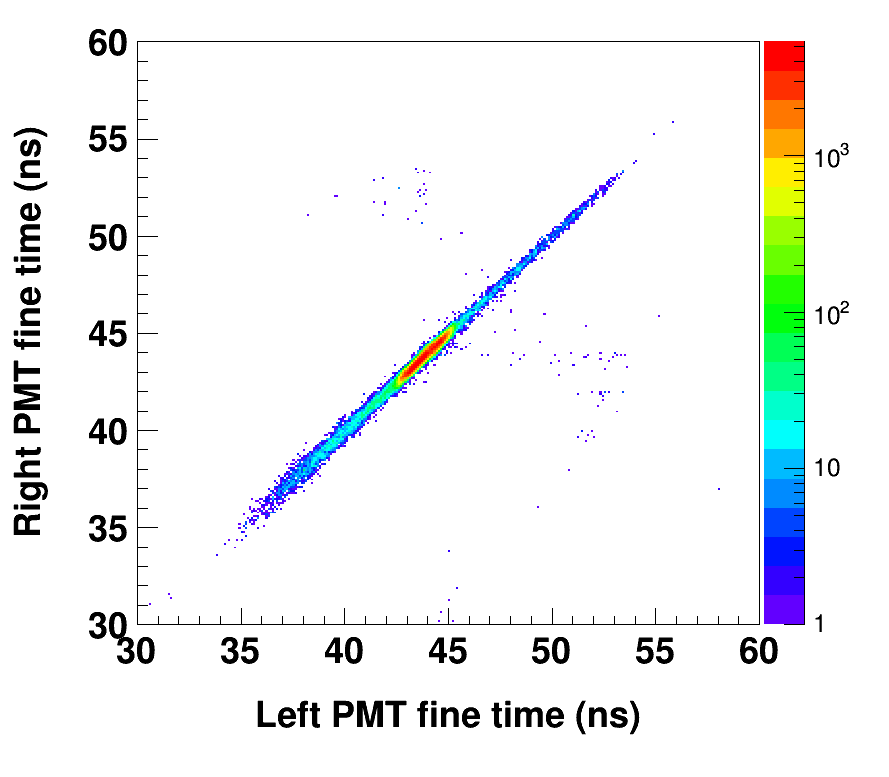
\includegraphics[width=0.8\textwidth]{figures/LRCorrelation.png}
    \caption[Event times for left and right PMTs of time-of-flight detector]
    {Fine times for left and right PMT events, taken separately, of the time-of-flight 
        detector as recovered by our software CFD algorithm. The times plotted are referenced
        to the start of each event waveform, which varied by several ns event-to-event.
        Thus the spread from 35-
        55 ns depends on where the digitizer initiated the waveform for each
        event and does not indicate timing resolution information.}
    \label{LRCorrelation}
\end{figure}

%\begin{figure*}
%    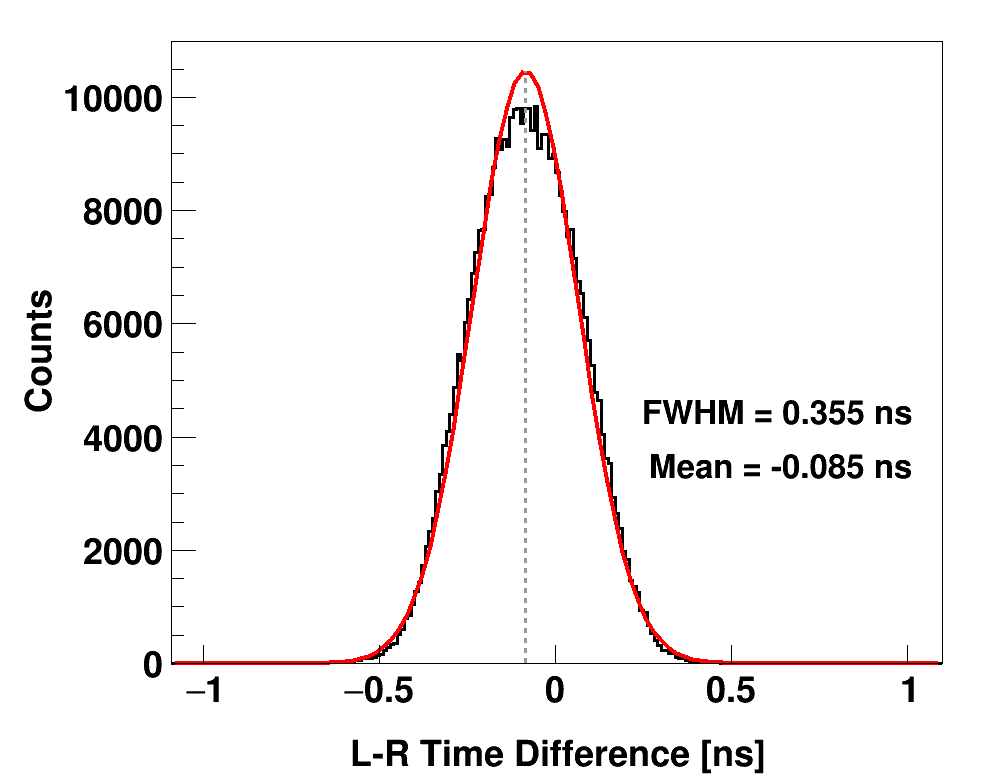
\includegraphics[scale=0.3]{figures/Difference_Linear.png}
%    \caption[Time difference between left and right PMTs of time-of-flight detector] {
%        For all events in a diagnostic run, the time difference   
%        between the left and right PMTs of the TOF detector is plotted.
%        A Gaussian fit (in red) to these events reveals an 85-ps delay of the right PMT with 
%        respect to the left PMT and a left-right time difference FWHM of 355 ps.
%    }
%    \label{LRTimeDifferenceLinear}
%\end{figure*}

\begin{figure}[h]
    \centering
    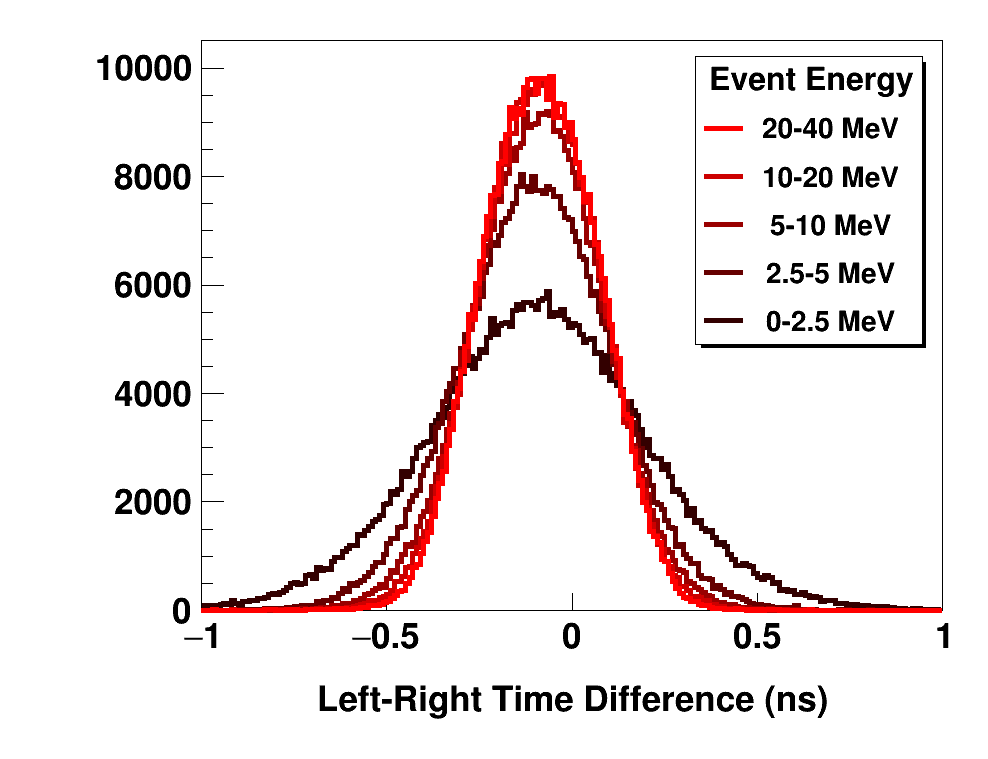
\includegraphics[width=0.8\textwidth]{figures/LRDifferenceByEnergy.png}
    \caption[Effect of energy gating on left/right PMT time difference]
    {Effect of energy gating on the left/right PMT time difference. Higher-energy neutrons 
    traverse also deposit more energy on average, slightly improving the
    precision of the software CFD. The same number of events are populated into
each histogram.}
    \label{LRTimeDifferenceByEnergy}
\end{figure}

\begin{figure}[h]
    \centering
    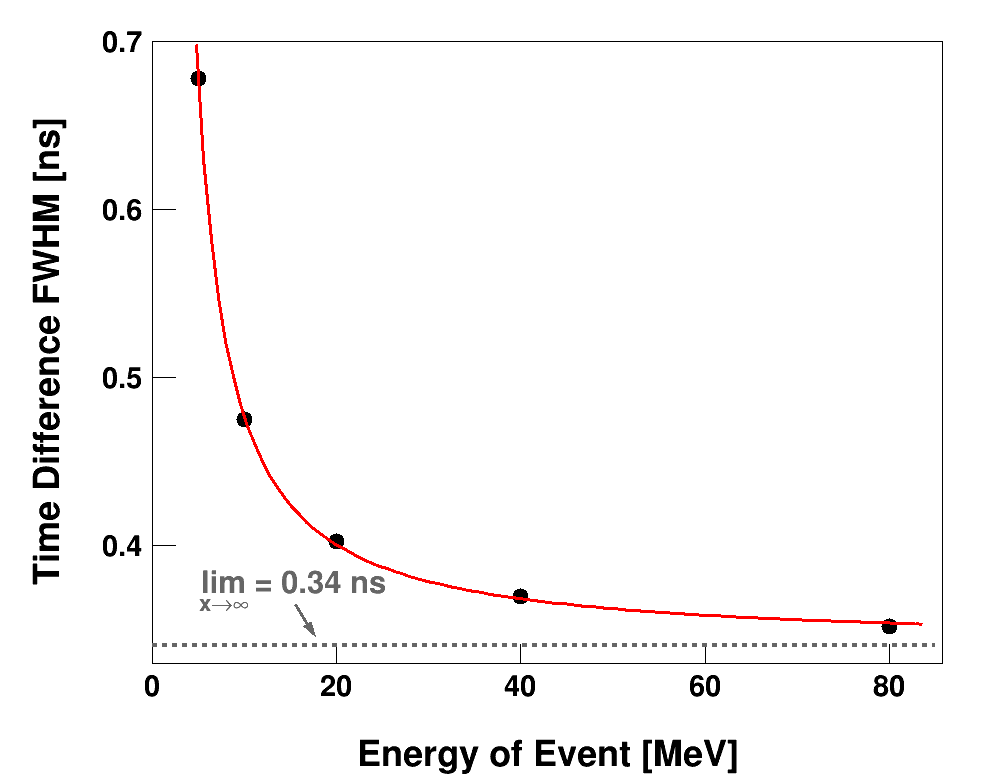
\includegraphics[width=0.8\textwidth]{figures/DifferenceThresholdsFit.png}
    \caption[Intrinsic time resolution of time-of-flight detector as a function
    of signal amplitude]
    {
        The time difference between the left and right PMTs
        of the TOF detector was calculated for all events in a diagnostic run.
        The FWHM of these time differences as a function of
        neutron energy are shown (black points) and fitted with a hyperbolic
        curve (red line). For low-energy
        events, the time resolution is poorer due to the lower signal amplitude.
        As energy increases, the FWHM time resolution asymptotically approaches 0.34
        ns (grey dashed line).
    }
    \label{DifferenceThresholdsFit}
\end{figure}

To calculate the time-of-flight for each event, the ``starting gun'' of each
micropulse had to be precisely determined. All event times were first adjusted for cable and 
electronics delay, so that each event was assigned to the correct macropulse.
To reduce unnecessary data collection, we collected only the first \tZero, a
logic signal, of each macropulse. 
Using this time and the precisely-known micropulse frequency, we identified all $\gamma$ rays 
for a given macropulse and tabulated
the average $\gamma$ time-of- flight, as shown in Fig. \ref{GammaCorrection}.
The uncertainty of our macropulse start time manifests as a spread in average gamma times-of-
flight. Were the start time exactly known for each macropulse, and the
micropulse period exactly known, the time-of-flight for each gammas should be
exactly the same, excepting the detector time resolution. Thus, the difference between the 
average calculated gamma times-of-flight (using the imprecise macropulse start
time) and the \textit{expected} TOF (given the TOF detector distance and speed of light)
can be used to improve the macropulse start time. This $\gamma$-averaging
procedure was applied to all events in each macropulse (see Fig.
\ref{TimingCorrectionStudy}). We also examined the stability of the \tZero\
period and found that its day-to-day variation had a negligible effect on the
calculated times-of-flight (see Fig. \ref{RFTimeStudy}).

After these corrections, the total time-of-flight
resolution, taken as the FWHM of the $\gamma$-ray peak in the time-of-flight
spectrum, ranged from 0.60-0.90 ns over the series of \tot\ measurements. This is comparable 
to the resolution from our digitizer-mediated Ca experiment from 2008 \cite{Shane2010},
which used a similar $\gamma$-averaging technique. For a 100-MeV
neutron and a time-of-flight detector distance of 27 meters, an
uncertainty of 0.80 ns translates to an energy resolution of $\approx$900 keV.
For neutrons below $\approx$20 MeV, the time-of-flight time resolution worsens as the 
traversal time through the 1-inch thickness of the scintillator becomes non-negligible.
However, because the time-of-flight of these neutrons is already several hundred ns or
longer, the relative energy resolution ($\frac{\Delta E}{E}$) is
superior at low energies. To wit, for a 5 MeV neutron with a 0.82 ns detector-traversal time and
an inherent TOF resolution of 0.80 ns, $\Delta E$ is only 13 keV. These energy uncertainties
have been propagated through the subsequent analysis.

\begin{figure}[h]
    \centering
    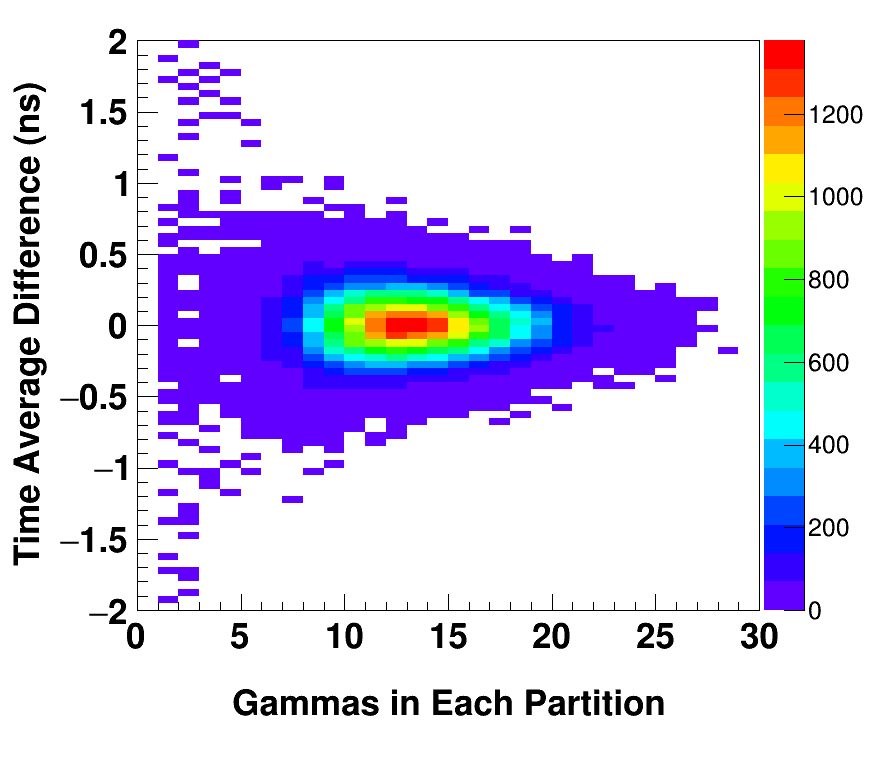
\includegraphics[width=0.8\textwidth]{figures/gammaCorrection2D.png}
    \caption[Deviation of the average $\gamma$-ray arrival time by macropulse]
    {Deviation of the average $\gamma$-ray arrival time by macropulse. }
    \label{GammaCorrection}
\end{figure}

\begin{figure}[h]
    \centering
    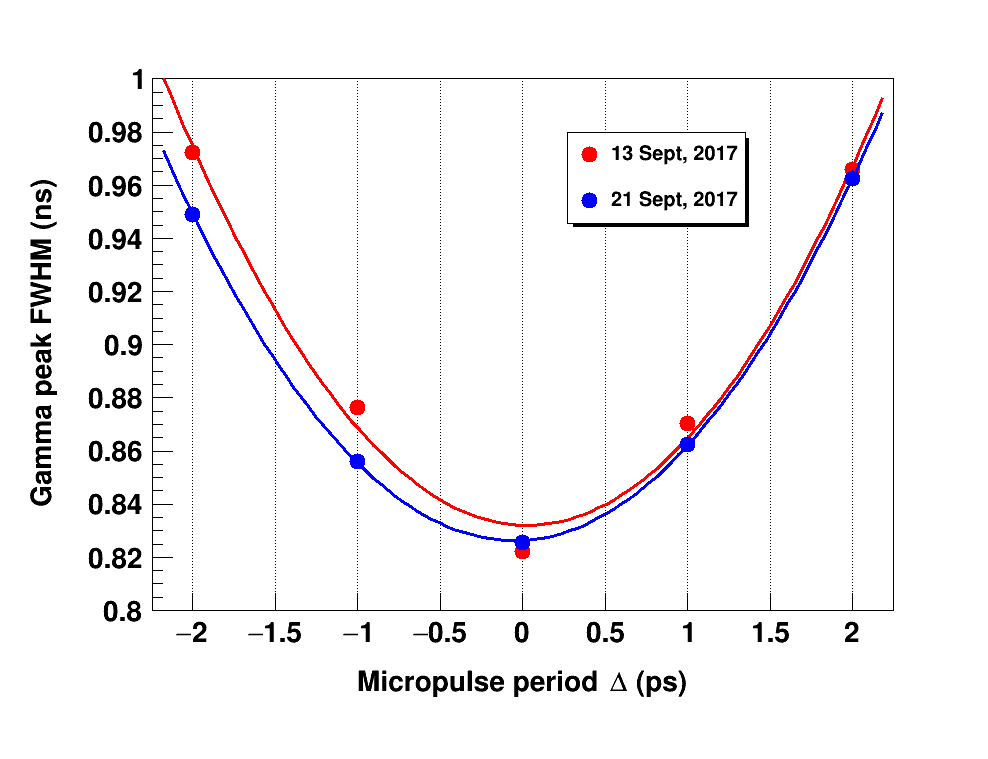
\includegraphics[width=0.8\textwidth]{figures/RFTimeStudy.png}
    \caption[Stability of the beam pick-off (T$_{0}$) during the experiment]
    {Results of a study of the micropulse frequency stability. The \tZero\ period used
        in the analysis was varied in 1-ps increments, changing the
        calculated arrival time of events in each micropulse. For each period, the FWHM of
        the time uncertainty in the $\gamma$-ray flash was tabulated, and the
        overall trend fitted with a quadratic curve. The true micropulse
        frequency was taken as the minimum of this curve. This procedure was
        repeated on data from different days throughout the experimental run,
        verifying that micropulse frequency drifting has a negligible effect
        on the recovered times-of-flight.
    }
    \label{RFTimeStudy}
\end{figure}

\begin{figure}[h]
    \centering
    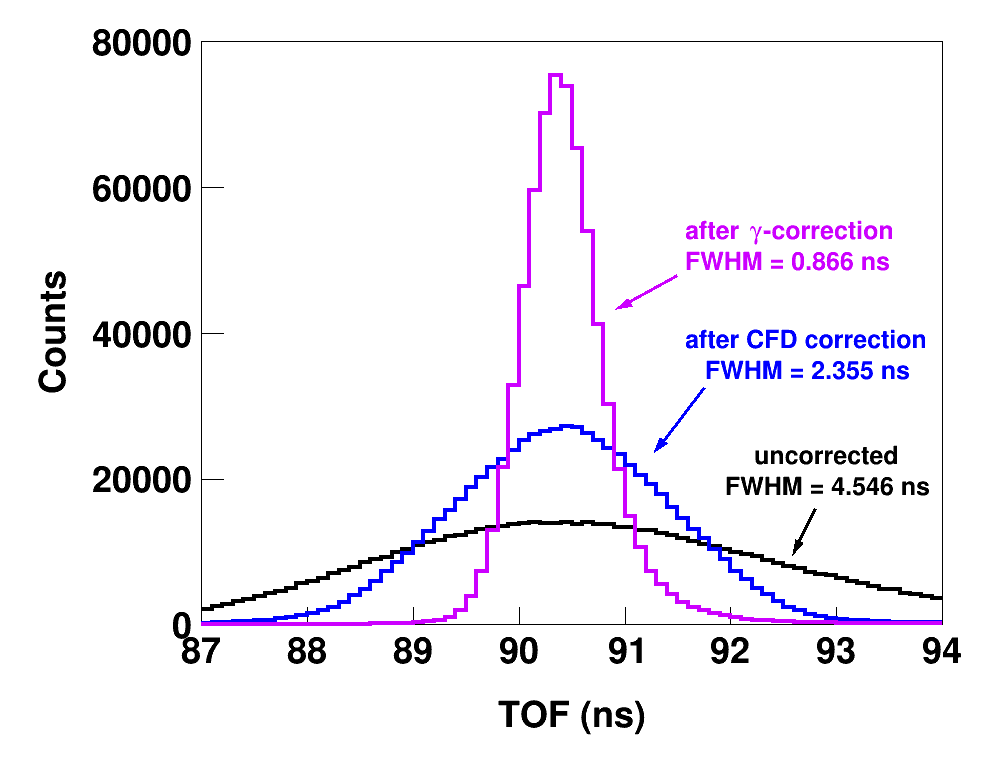
\includegraphics[width=0.8\textwidth]{figures/TimeCorrections.png}
    \caption[Improving timing precision with a software CFD and $\gamma$-ray averaging]
    {The effects of timing corrections on the $\gamma$-ray
        peak of a typical run are shown. The uncorrected spectrum is shown in black,
        the spectrum after correction with our software CFD is shown in blue,
        and the spectrum after correction with both our software CFD and
        $\gamma$-averaging is 
        shown in pink. For this run, the final $\gamma$-ray peak 
        FWHM after both corrections is 0.866 ns, comparable to the precision we
        achieved in our Ca study \cite{Shane2010}, which also employed $\gamma$-
        averaging.}
    \label{TimingCorrectionStudy}
\end{figure}

Precise determination of the TOF distance was done by comparing our measured \tot\ data
for $^{\text{nat}}$C with the precisely known resonance structure from 3-15 MeV
(Fig. \ref{DistanceStudy}). The distance was determined as 2709$\pm$1 cm for the
Ni and Rh run configuration and 2554 $\pm$1 cm 
for the Sn and O run configuration. With all corrections applied, all events in the 
time-of-flight detector channel were filtered against events in the veto detector to remove
events caused by charged-particles created along the flight path.

\begin{figure}[h]
    \centering
    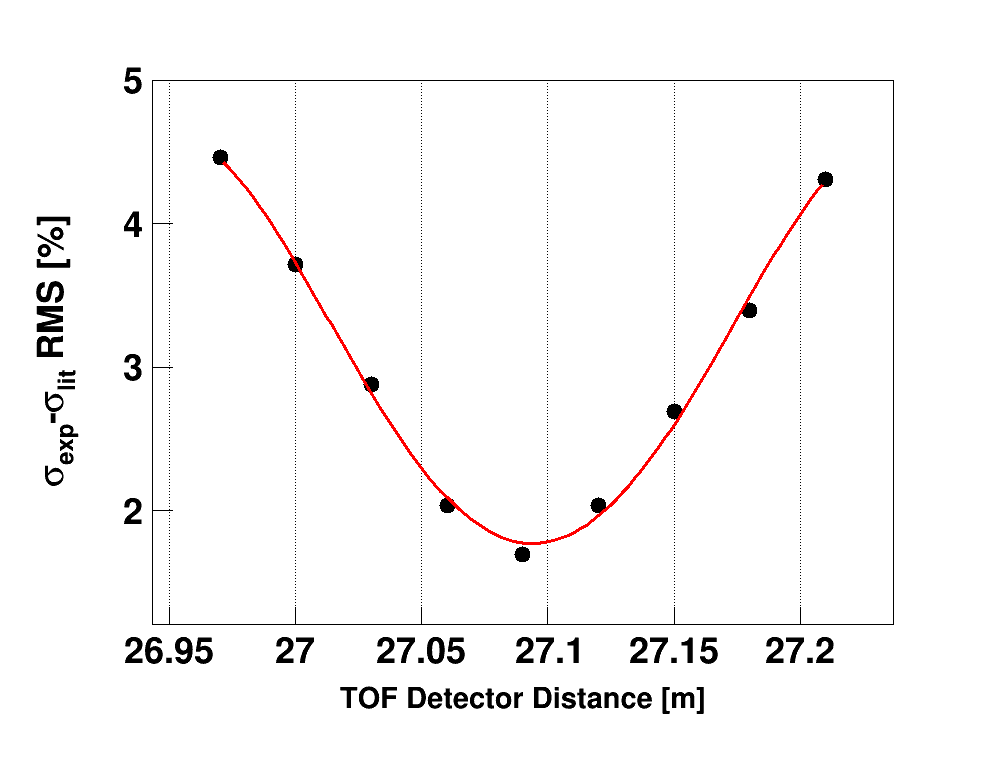
\includegraphics[width=0.8\textwidth]{figures/DistanceStudyNi.png}
    \caption[Determining the time-of-flight detector distance using \cNat\ resonances]
    {Results of a study to determine the distance between
    the neutron source and the TOF detector for the Ni/Rh running configuration
are shown. First, a plausible range of flight path distances (26.97-27.21 m) was
selected based on rough estimation during the experiment. Using each
distance in this range, the \tot\ for natural carbon was calculated in the
resonance region (3-15 MeV). The RMS difference between the cross section
generated using that distance and literature data from Abfalterer
\cite{Abfalterer2000, Abfalterer2001} was calculated (shown as black points in
the figure). A quartic fit to these RMS data is shown (solid line). By minimizing the
RMS difference, the flight path distance of 2709$\pm$1 cm was determined for the
Ni and Rh run configuration.}
    \label{DistanceStudy}
\end{figure}

\section{Deadtime Correction} \label{DeadtimeCorrection}
Because events are not processed instantaneously, there is a brief period
after each trigger during which the digitizer is busy processing that trigger.
 The busy period following each event is referred to as the ``analytic" or ``per-event" deadtime and can be corrected for according to standard techniques \cite{Moore1980}.
In an ideal experiment, the instantaneous flux at all times would be
sufficiently low (and the amount of beam time available sufficiently high) that
only very rarely would another event arrive at the time-of-flight detector while
a previous event was still being processed. In reality, given the low duty
factor of the pulsed beam, the flux during each pulse must be high to achieve sufficient
statistics over dozens or hundreds of energy bins within a few weeks of beam
time. Given the extremely small areal density of our targets, this meant a rate
of approximately one event per micropulse on average. Even with a flat
time-of-flight spectrum, a sizable fraction of events would arrive in the shadow
of the previous event's processing period, and thus be ignored by the pulse-processing firmware.
In reality, the
problem is far worse, as the instantaneous flux is much higher during the gamma
flash and arrival of high-energy neutrons.

In \cite{Finlay1993, Abfalterer2001}, this problem was addressed by using a
``looking period" logic. Arriving T$_{0}$ signals were used to begin a ``looking 
period" during which neutron and $\gamma$-ray
events could be collected. At the time of the T$_{0}$ arrival, if the electronic modules
were still busy from processing a previous event (as indicated by a "system busy" signal),
the looking period was aborted. During a looking period, if a single neutron or gamma
was detected, no subsequent events were allowed in the period.
This logic is diagrammed in Fig. \ref{AnalogLogic}, reproduced from
\cite{Abfalterer2001}. The fraction of T$_{0}$ signals that result in looking
periods ($\frac{T_{0,live}}{T_{0}}$) is tabulated, as is the so-called ``analytic dead-time'', i.e. 
the chance that the detector is busy for a given time \textit{within each looking period}.
Time-of-flight histograms are then scaled by these
fractions to recover the true number of events per unit flux. This approach is useful if the
analytic deadtime is commensurate with the micropulse period, as it means that
only one event can be detected per micropulse anyway. For this approach to be successful, the
analytic dead-time must be very precisely known, as corrections can soar to over 100\%
if the beam flux is high.

\begin{figure}[h]
    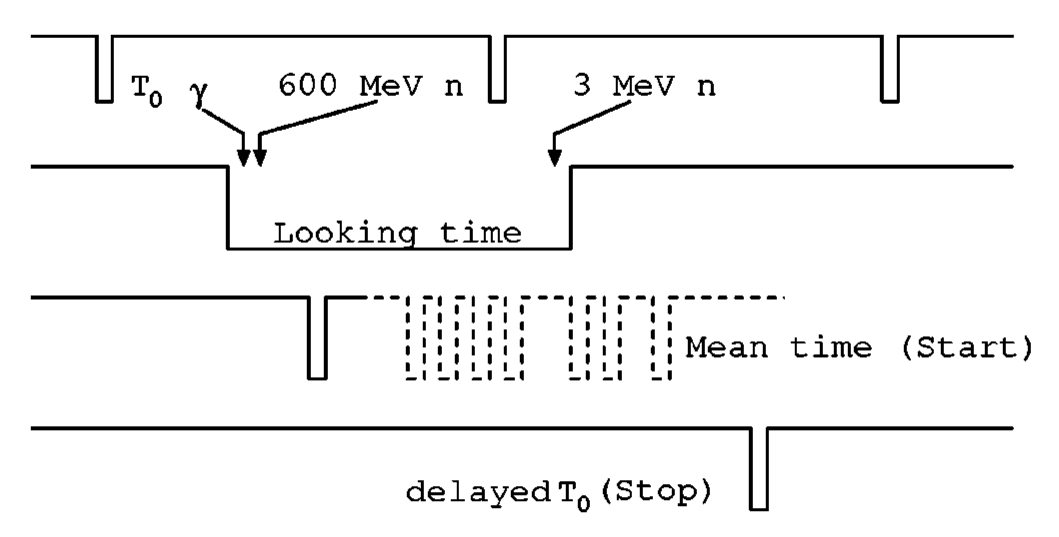
\includegraphics[width=0.45\textwidth]{figures/AnalogLogic.png}
    \caption[``Looking period'' logic used by previous neutron \tot\ measurements at LANSCE]
    {
        ``Looking period'' logic used by previous neutron \tot\ measurements at LANSCE
        \cite{Abfalterer2001}. Per the original caption: proton beam bursts arriving at
        evenly-spaced 1.8-$\mu$s time intervals define a time frame 1.4-1.6 $\mu$s long. For each
        time frame, a delayed copy of the \tZero\ defining it was used as a stop signal on the TDC
    clocks.}
    \label{AnalogLogic}
\end{figure}

Due to the extremely low areal density of our samples,
we could not afford to discard any neutron events and still acquire sufficient statistics. 
Thanks to the dramatically-reduced analytic deadtime of the digitizer algorithm,
we could use a more straightforward deadtime correction logic and minimize the
number of lost events. Assuming negligible variation in beam flux between micropulses
(an assumption investigated below), the fraction of time $F[i]$ that the digitizer is dead 
for a given time bin $i$ can be calculated:

\begin{equation}
    F_{i} = \sum^{N-1}_{j=0} R_{(i-j)\text{ mod N}}\times P_{j}
\end{equation}

\noindent
where $N$ is the number of time bins in the micropulse, $R_{x}$ is the rate of
detected events per micropulse in bin $x$, and $P_{j}$ is the probability that the
digitizer is still busy from a trigger $j$ bins ago. Moore \cite{Moore1980} also provides
a more advanced 
formula to generate the appropriate dead-time correction in cases where the variation in beam 
flux is significant. However, an examination of our flux-per-micropulse data 
showed almost no variance in the flux per micropulse, except during the first 10\%
of each macropulse when flux was "ramping up". In our final analysis, we have discarded the 
first 40 micropulses of each macropulse and used the simpler Eq. \ref{DeadtimeEquation} to 
calculate the dead-time fraction.

To model $P_{j}$, we
employed a logistic function and fitted it to the observed spectrum for time
differences between consecutive events (see Fig.  \ref{TimeDifferenceBetweenEvents}).
For a given bin $i$, the fraction of time that the 
digitizer is dead, $F_{i}$, is in essence a discrete convolution of the
\textit{measured} TOF spectrum with $P_{j}$. Note that except for the first and
last micropulses in a macropulse, micropulses are consecutive and thus deadtime effects can
``wrap around" from the end of one micropulse to the next. For these wrap-around
contributions (that is, $j>i$), the (mod N) term ensures that the bin referred
to by $i-j$ is non-negative and has physical meaning as a time bin from the previous 
micropulse.

By optimizing trigger processing in digitizer firmware,
we reduced the per-event deadtimes affecting our
measurement ranged from 150-230 ns depending on the digitizer configuration.
For a 230 ns per-event deadtime, the probability-dead
$F_{i}$ of our time bins is given in Fig.
\ref{ExampleDeadtimeSpectrum}, showing that the probability-dead never exceeds
25\%, much smaller than the 50-80\% typical in the approach described above
\cite{Finlay1993, Abfalterer2001}.
Once the fraction dead was identified for each time bin, the total number of
events detected in that bin, $N_{m}[i]$, was corrected to the \textit{true}
number of events in that bin $N_{t}[i]$ that would have been detected in the
absence of a per-event deadtime:

\begin{equation} \label{DeadtimeEquation}
    N_{t}[i] = -ln\left(\frac{1-\frac{N_m[i]}{M}}{(1-F_{i})\times M}\right)
\end{equation}

\noindent
where M is the total number of micropulse periods. The difference between
uncorrected and analytic-deadtime-corrected TOF spectra is shown in Fig.
\ref{CorrectionEffectOnTOF}. At large TOFs (low energies) the correction is as low as a
few percent, but at small TOFs (high energies) when the digitizer is still dead
from the $\gamma$-ray flash and high-energy neutrons, the correction is significant
($\approx$20\% for our Ni/Rh runs, and $\approx$40\% for our Sn/O runs). Again, these 
corrections are themselves far lower than the correction required
when using the previous approaches \cite{Finlay1993, Abfalterer2001}, which
could be over 100\% for the lowest-energy neutrons, depending on beam flux. It is
important to keep in mind that in these experiments the dead time is not a fixed number but a
function of the neutron energy.

\begin{figure}[h]
    \centering
    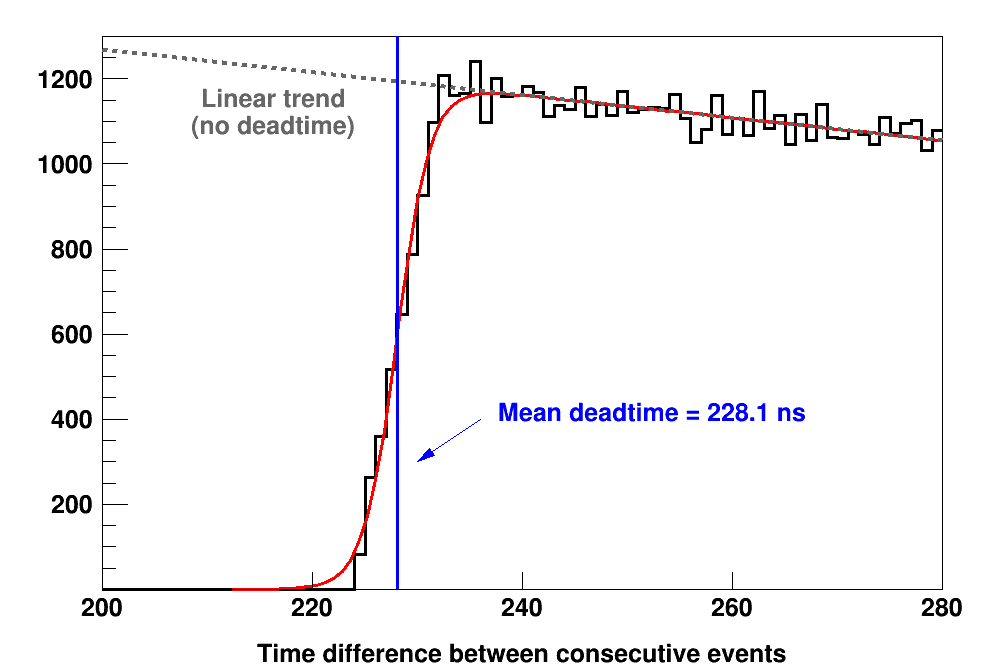
\includegraphics[width=0.8\textwidth]{figures/TimeDifferenceBetweenEvents.png}
    \caption[The time difference between consecutive events in the time-of-flight detector]
    {The time difference between adjacent TOF-detector
    events for a single run is plotted (black histogram). Below a certain
minimum time difference (the ``deadtime"), no events are recorded. A logistic
fit (red) models the detector's deadtime response and is used to generate a
deadtime correction. The underlying linearly-decreasing count rate (gray dashed
line) in incorporated into the logistic model. From the fit, a mean deadtime of
228.1 ns was extracted for the Sn and O run configurations (a similar
procedure was used to recover a deadtime of [insert deadtime] for the Ni and Rh
run configurations).}
    \label{TimeDifferenceBetweenEvents}
\end{figure}

\begin{figure}[h]
    \centering
    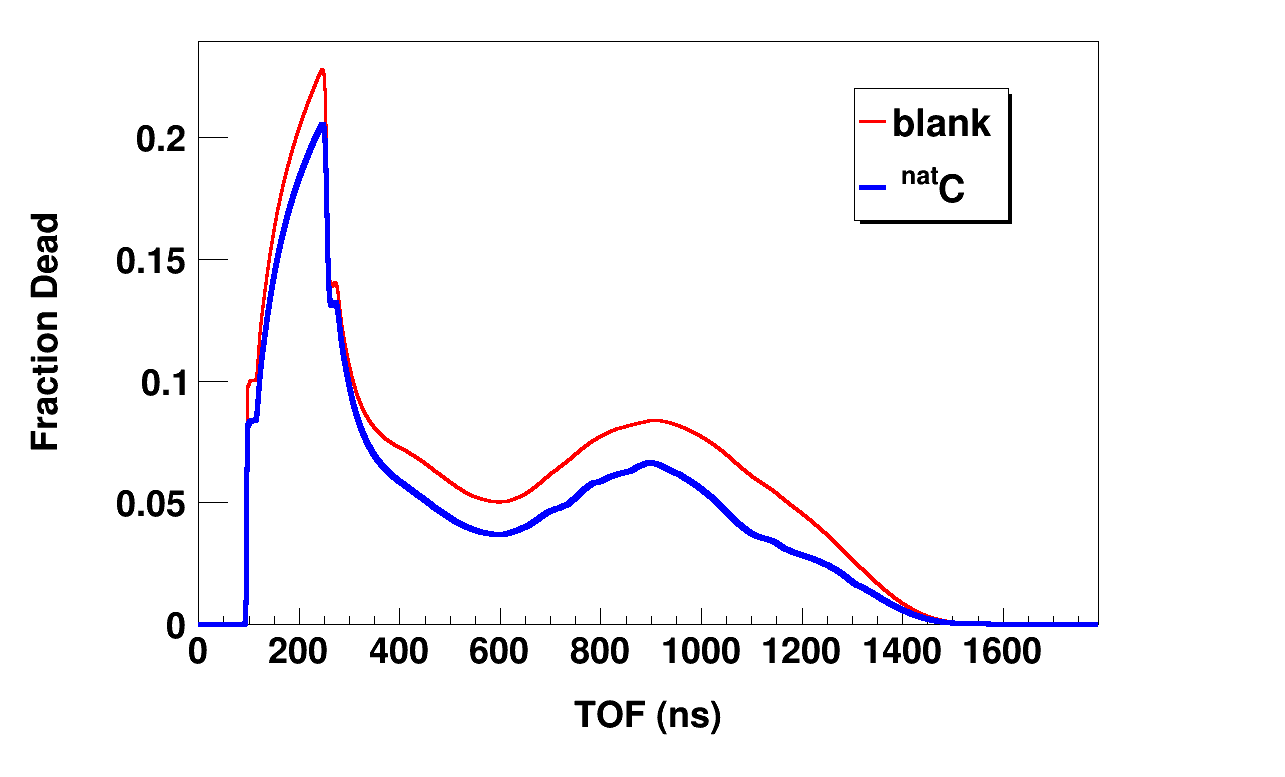
\includegraphics[width=0.8\textwidth]{figures/exampleDeadtimeSpectrum.png}
    \caption[Digitizer busy probability as a function of time within micropulse]
    {Using TOF data from a typical run, the probability that a given 
        TOF bin is ``dead" is shown for the blank sample (dashed line) and the 
        $^{\text{nat}}$C   
        sample (solid line). The sharp rise at 90 ns is the response to the
        $\gamma$-ray flash, the gradual increase from 90-245 ns is the response to
        the arrival of high-energy neutrons, and the sharp fall at 245 ns
        is the elapse of the $\gamma$-ray ``shadow". Only high-energy neutrons
        have a probability-dead exceeding 10\%.}
    \label{ExampleDeadtimeSpectrum}
\end{figure}

\begin{figure}[h]
    \centering
    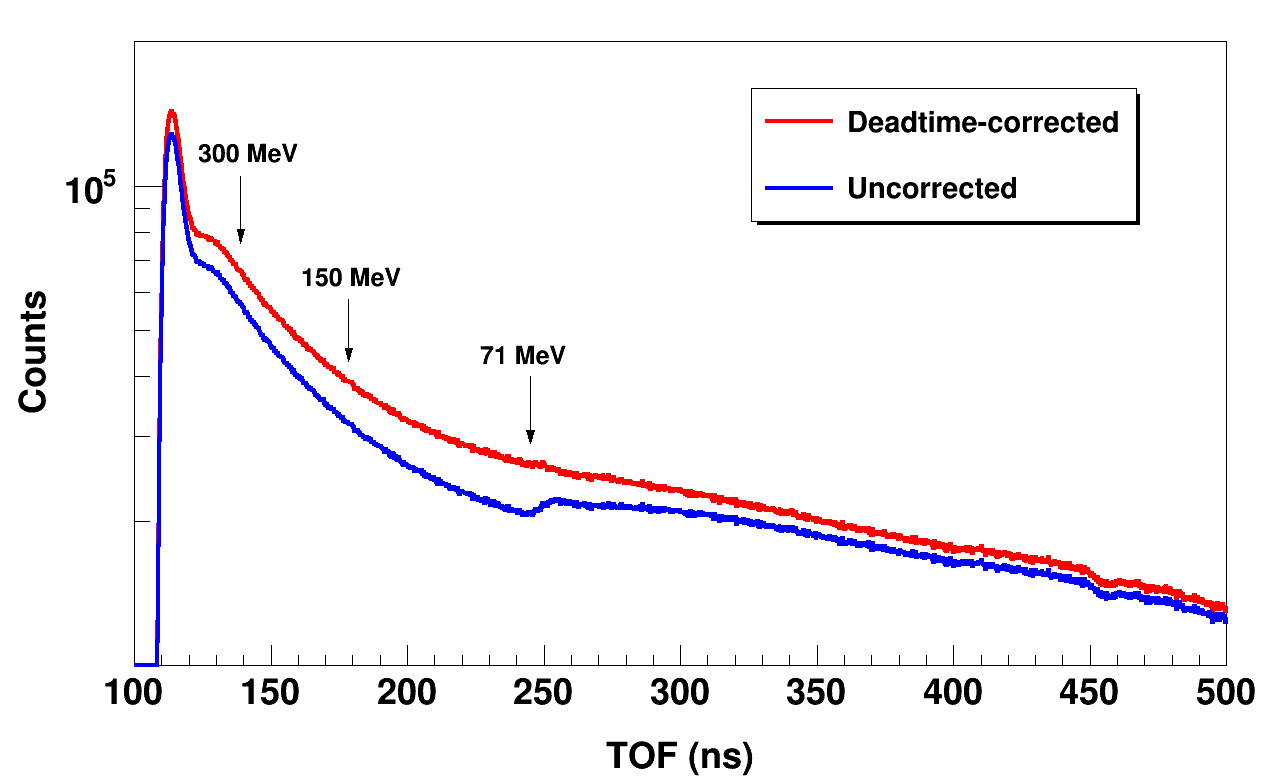
\includegraphics[width=0.8\textwidth]{figures/CorrectionEffectOnTOF.png}
    \caption[The effect of deadtime correction on a typical time-of-flight spectrum]
    {A typical TOF spectrum from the Ni/Rh
        run configuration is shown, before (in blue) and after (in red) analytic
        deadtime correction. Relevant neutron energies are indicated above the spectra.
        For this digitizer configuration, the mean deadtime was 155 ns (see Fig.
        \ref{TimeDifferenceBetweenEvents} for details on mean deadtime determination).
        Note that at 245 ns, there is an
        obvious defect in the uncorrected spectrum is repaired in the corrected
        spectrum. The defect
        corresponds to the elapse of the 155-ns-long deadtime ``shadow" from the $\gamma$-ray
        flash, which arrived at 90 ns (not shown).}
    \label{CorrectionEffectOnTOF}
\end{figure}

During analysis, it was noted that occasionally (1 in 400 macropulses), one or two 
adjacent macropulses would have an abnormally small number of flux monitor events or 
TOF events. The frequency of these ``data dropouts" was similar to the rate of
switching between DPP and waveform modes and we suspect it is related to edge
case behavior right before or after a mode switch. To mitigate this issue,
any macropulse that had less than 50\% of the average event rate in either the
flux monitor or TOF detector channel was ignored.

After applying these corrections, the veto and integrated charge gates are applied to 
all events and surviving events are populated into time-of-flight spectra (see Fig.
\ref{ExampleTOFSpectrum}). From these spectra, room background was subtracted
(responsible for 0.1\% to 1\% of event rate, depending on energy)
and events were mapped to the energy domain.

\begin{figure}[h]
    \centering
    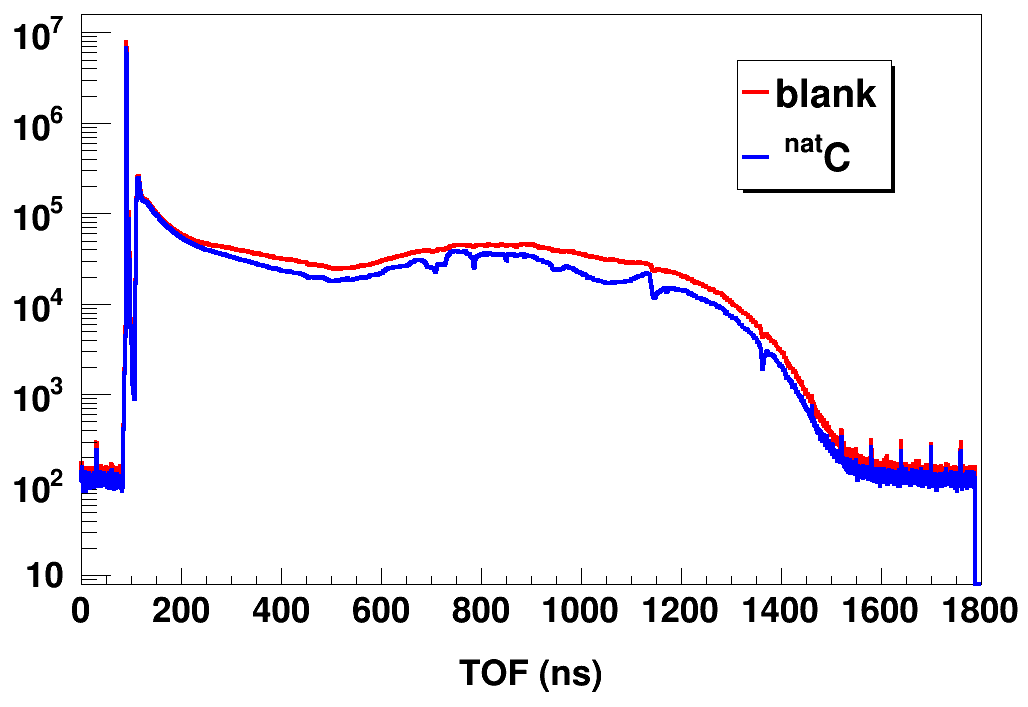
\includegraphics[width=0.8\textwidth]{figures/exampleTOFSpectrum.png}
    \caption[Typical time-of-flight spectrum after timing and deadtime corrections]
    {
        Typical time-of-flight spectra after analytic deadtime correction and
        veto and integrated charge gating. A spectrum from the blank sample is shown in
        red and a spectrum for the $^{\text{nat}}$C sample is shown in blue, both from the Ni/Rh 
        experiment configuration.
        The $\gamma$-ray peak presents as a sharp spike at 90 ns, followed by
        the highest-energy neutrons at 130 ns. The small spikes spaced 60 ns
        apart (visible before 90 ns and after 1500
        ns) are $\gamma$-ray peaks from a low-level, continuous ``drip" 
        of protons onto the tungsten target caused by mistuning of the proton 
        buncher; their effect on the calculated cross sections is negligible. Low-energy carbon
        resonances are visible above 600 ns.
    }
    \label{ExampleTOFSpectrum}
\end{figure}

It is worth mentioning two additional systematic differences between our configuration and
those of previous LANSCE measurements \cite{Shane2010, Finlay1993, Abfalterer2001}, namely the
flight path length and sample diameters. Flight path lengths of 37.70 meters, 38.14 meters, and 45
meters were used in \cite{Finlay1993}, \cite{Abfalterer2001}, and \cite{Shane2010} respectively, 
much longer than the 25-27 meters position of our time-of-flight detector.
Had these lengths been available for our experiment,
it would have reduced the high-energy instantaneous neutron flux by 
$\frac{1}{3}$, potentially affecting our results for the highest-energy neutrons. Future
experimental work at the 90 meter flight path station at LANSCE would be ideal: the
instantaneous neutron flux would be reduced by more than half compared to our experiment
and neutrons as low as 10 MeV could still be unambiguously identified before micropulse wraparound.
The other major difference, the sample diameters, affects the diameter of the collimation used.
Diameters of  2.2-2.9 cm, 2.3-3.8 cm, and [insert Shane] were used for \cite{Shane2010},
\cite{Finlay1993}, and \cite{Abfalterer2001}, respectively, much larger than the 0.8 cm diameter of
our samples. As sample (and thus collimator) size decreases, the cross-sectional area of the
collimation pipe decreases compared to its circumference. At some point, neutrons scattering to very
small angles on the interior of the collimation could become significant compared to the number of
neutrons passing through the collimation freely. While we do not expect this phenomenon to affect
our results, at smaller collimation diameters, a collimation-scattering simulation may be warranted.

\section{Cross Section Calculation}
The fundamental quantity of interest, \tot, is related to the flux
loss through a sample by:

\begin{equation}
I_{t} = I_{0}e^{-{\ell\rho\sigma_{tot}}}
\end{equation}
or, equivalently,
\begin{equation}
    \tot = -\frac{1}{\ell\rho}ln\left(\frac{I_{t}}{I_{0}}\right)
\end{equation}

\noindent
where $I_{0}$ is the neutron flux entering the sample, $I_{t}$ is the neutron
flux transmitted through the sample without interaction, $\rho$ is the number
density of nuclei in the sample, and $\ell$ is the sample length. For thin
or low-density samples, flux attenuation through the sample will be small
(e.g., 13\% for our Ni samples at 100 MeV) and a large number
of counts will be required to determine the cross section to high
precision.

From these energy spectra, the raw cross sections were calculated, bin-wise, as follows:
\begin{equation} \label{CSCalculation}
    \tot = -\frac{1}{\ell\rho_{n}}
    \ln \left(\frac{I_{0}}{I_{s}}\times\frac{M_{s}}{M_{0}}\right)
\end{equation}
where $\frac{I_{0}}{I_{s}}$ is the ratio of counts in the energy spectra between 
the blank and sample, $\frac{M_{s}}{M_{0}}$ is the ratio of counts in the
monitor detector between the sample and blank (for flux normalization), $\ell$ is the length 
of the sample, and $\rho_{n}$ is the number density of atoms in the sample.

%To compare \tot\ for two different targets of masses A and A', the relative
%difference \totRD\ is useful:
%\begin{equation} \label{SASRelDiff}
%    \begin{split}
%        \totRD & \equiv
%    \frac{\sigma_{A}-\sigma_{A'}}{\sigma_{A}+\sigma_{A'}} \\
%    & =
%    \frac{r_{0}^{2}(A^{\frac{2}{3}}-A'^{\frac{2}{3}}) +
%    2\lambdabar r_{0}(A^{\frac{1}{3}}-A'^{\frac{1}{3}})}
%    {r_{0}^{2}(A^{\frac{2}{3}}+A'^{\frac{2}{3}}) +
%    2\lambdabar r_{0}(A^{\frac{1}{3}}+A'^{\frac{1}{3}}) + 2\lambdabar^{2}}
%    \end{split}
%\end{equation}

A series of small corrections were applied to the raw cross sections to produce
the final results. First, because the blank sample contains air and not vacuum,
the cross section of air must be added to each other sample's cross section (scaled by  
the ratio of areal densities of air in the blank and the sample of interest).
For the \rhThree\ sample, which had the smallest areal density, this correction
was approximately 2 mb $>$100 MeV. The cross section for $^{64}$Ni was corrected for the 
isotopic enrichment of our
sample (92.2\%) using our measured $^{\text{nat}}$Ni cross section. All other isotopes were 
sufficiently pure such that the isotopic impurities contributed $<$0.1\% to the final
cross section.

Oxygen cross sections were calculated by
subtracting the well-known hydrogen cross section from the raw H$_{2}$O result
(we used H \tot\ data sets from Clement et al \cite{Clement1972} and Abfalterer
et al \cite{Abfalterer2001}, which together cover the range $0.5 \leq E_n \leq 500$ MeV
and are in excellent agreement where their energy ranges overlap). In light of
the additional uncertainty inherent to this kind of subtractive \tot\
determination, a D$_{2}^{\text{nat}}$O sample from which the literature \tot\ for
D$_{2}$ could be subtracted was prepared as an additional cross-check. The
results of the deuterium-to-hydrogen relative difference are shown in Fig. \ref{DtoH}. 

\begin{figure}[h]
    \centering
    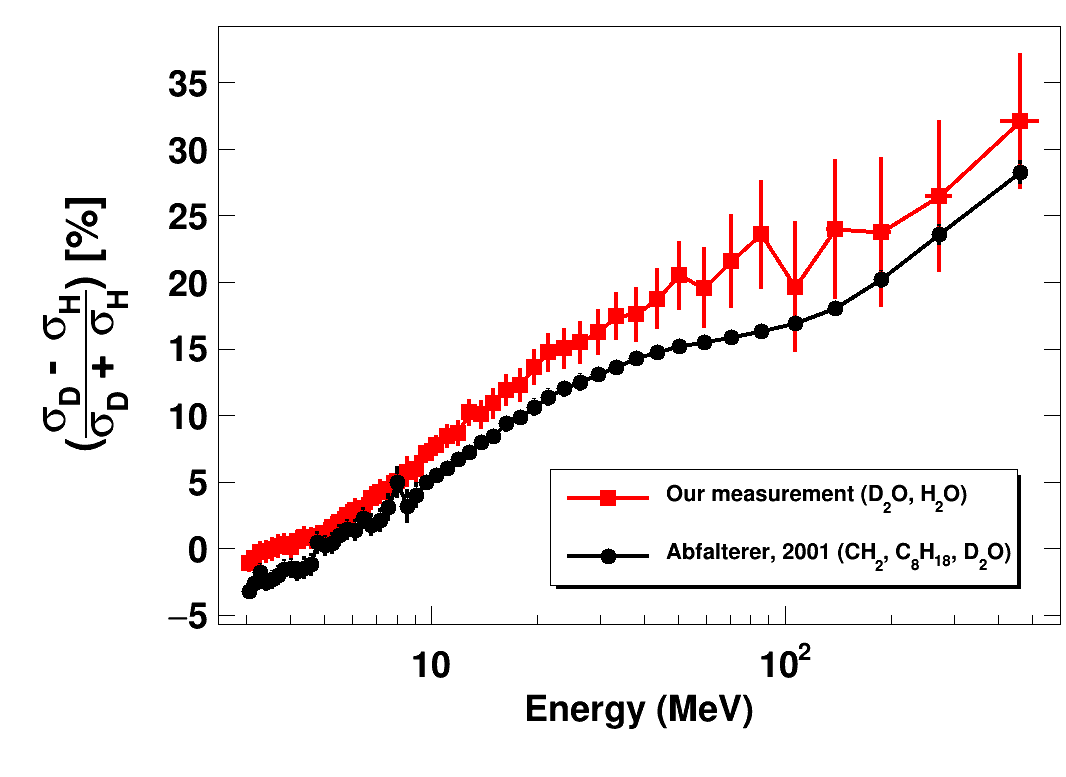
\includegraphics[width=0.8\textwidth]{figures/relativeDiff_DtoH.png}
    \caption{(Color online) Relative difference of cross sections of
        deuterium to hydrogen, as calculated by subtraction of our O \tot\ from
        D$_{2}$O and H$_{2}$O. Our results are shown in red; the measurement of
        Abfalterer et al. \cite{Abfalterer1998} is shown in black.}
    \label{DtoH}
\end{figure}

\section{Results}
\subsection{Benchmarking \tot\ results with natural samples}
To validate our analysis, we first compared our \tot\ measurements on natural samples
(\cNat, \niNat, \snNat, \pbNat) against the high-precision data sets on natural samples from 
Finlay et al. \cite{Finlay1993} and Abfalterer et al. \cite{Abfalterer2001}, shown in Fig.
\ref{LiteratureBenchmarking}. From 3-100 MeV, our measurements are in excellent
agreement, within statistical error, with these previous data sets. Above 100 MeV, our results 
diverge from the previous measurements, up to a relative difference of 5\% at 300 MeV for all 
targets) suggesting a small systematic effect at high energies, when the instantaneous neutron 
flux is highest. To investigate this discrepancy, we analyzed data from multiple digitizer 
thresholds during data production, applied various software threshold, gated events by low- 
and high-integrated charge, and varied our software CFD logic, among other diagnostic tests. 
Throughout these exercises, the agreement at $<$100 MeV and the discrepancy $>$100 MeV 
persisted. To ensure the shift was not related to imprecision in the areal
density of the targets, we compared both our short and long natural carbon targets against 
each other (see Fig. \ref{CarbonBenchmarking}) and found excellent agreement: the relative 
difference was within 1\% throughout our energy domain, comparable to a similar test
conducted by Abfalterer et al \cite{Abfalterer2001}. From Eq. \ref{CSCalculation},
it is clear that changes in flux ratio and sample areal
density can shift the calculated cross section up or down across the entire
energy range measured, but cannot change the \textit{slope} of the cross section
as energy is increased. Thus, the high-energy discrepancy is unlikely to be from
an incorrect monitor flux. Further, it was not dependent on the nuclear mass of
the sample nor with any other physical characteristics of the samples,
suggesting that backshine of neutrons into the flux monitor from the samples, or another 
physical mechanism, was not the cause.

At neutron times-of-flight corresponding to energies $>$100 MeV, the number of
counts in the spectrum rises sharply as one moves to higher energies. In this
region, even a sub-nanosecond timing differences between the spectrum for the
blank and for the sample of interest is amplified into large errors in the
cross section calculation. Thus the event timing and data
storage routines must be kept completely ignorant of which target is currently
in-beam so as to avoid sample-dependent timing effects. In practice, this is
difficult, as acquisition with the blank sample is naturally associated with
a higher data rate as fewer neutrons are absorbed or scattered in-flight than during
with samples in the beam path. By reducing the rate of data acquisition
by an order of magnitude or more, the analog-electronics approach reduces the
absolute data rates of both the blank and the samples, mitigating this effect.
However, because much larger samples are required with the overall reduced data
rate, the relative data rate between the blank and samples is increased,
amplifying any effect on the electronics. Without a study of digital and analog
systems running simultaneously with input from the same detectors, it is not
clear which approach suffers more from this effect. Such a follow-up, especially
with multiple digitizers from differing manufacturers, would help
resolve the high-energy discrepancy we see between all of our \tot\ data sets
and literature data.

\begin{figure}[h]
    \centering
    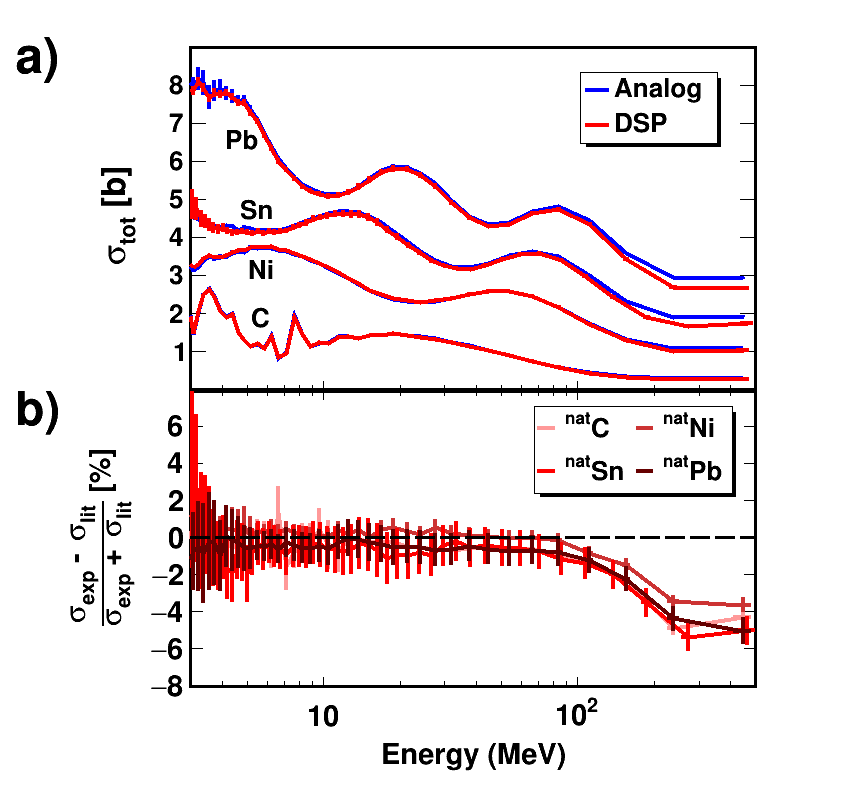
\includegraphics[scale=0.5]{figures/literatureBenchmarking.png}
    \caption[Comparison of our natural-sample \tot\ measurement against literature data]
    {
        A comparison of literature data (taken with analog
        techniques) and our results (signals processed with a digitizer, or "DSP")
        for natural C, Ni, Sn, and Pb. In panel a), the absolute cross sections are shown from
        3-500 MeV; in panel b), the relative differences between the literature data and
        our data are shown in percent. From 3-100 MeV, our data are fully consistent with the
        literature datasets but above 100 MeV, a relative difference arises, peaking at
        $\approx$5\% at 300 MeV.
    }
    \label{LiteratureBenchmarking}
\end{figure}

\begin{figure}[h]
    \centering
    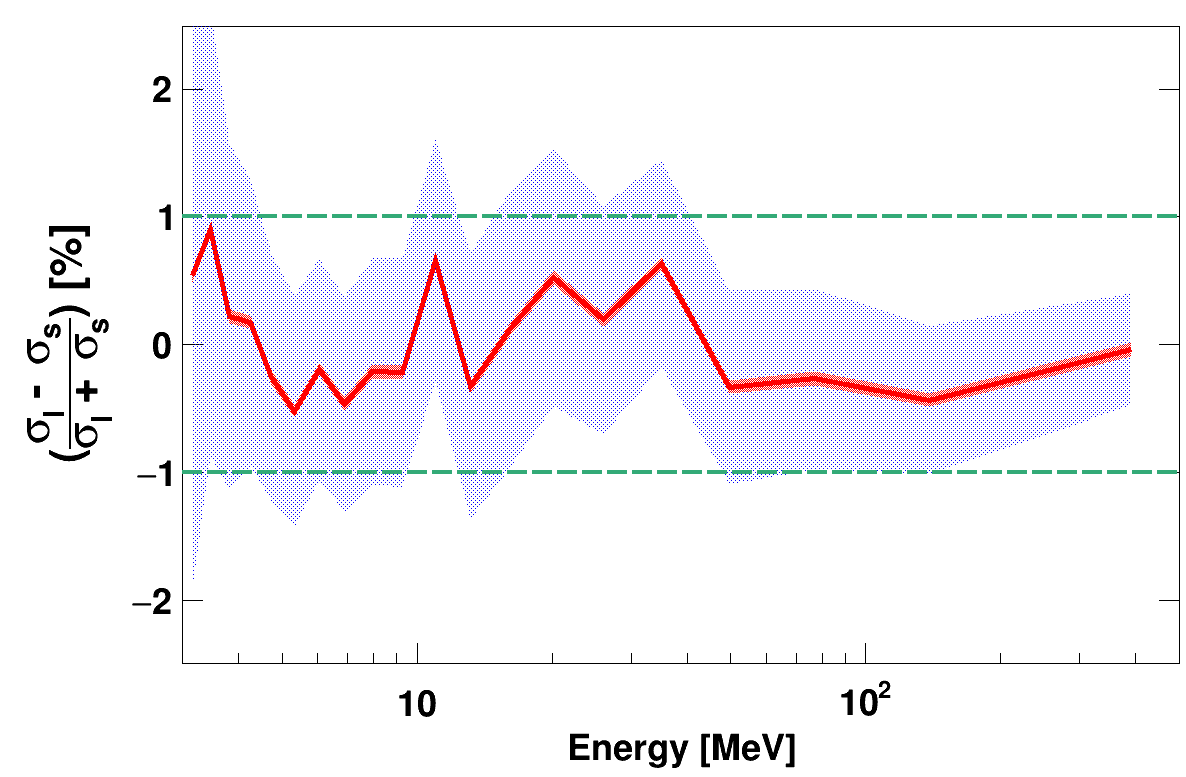
\includegraphics[scale=0.30]{figures/relativeDiff_longCarbonShortCarbon.png}
    \caption[Neutron \tot\ relative difference between short and long \cNat\ samples]
    {
        Relative difference of cross sections (red line) of
        our two lengths of \cNat, (27.3 mm and 13.7 mm), shown from 3-400
        MeV. Total error
        (including statistical and systematic) is indicated by the blue
        dotted region. Systematic error only (due to uncertainty in the areal
        density) is shown by the red hatched region (very small and immediately adjacent to 
        the red line). Clearly, statistical error dominates for this relative
        difference.
        Despite the low statistics of this diagnostic run (only 1.5 hours
        beam-on-target for each sample), the high efficiency of the
        digitizer-enabled approach means that the relative difference can be resolved to 
        $\pm$1\% for most of the energy range.
    }

    \label{CarbonBenchmarking}
\end{figure}

Our absolute \tot\ results for all isotopic targets are shown in Figs.
\ref{TwoPanelO}, \ref{TwoPanelNi}, \ref{TwoPanelRh}, and \ref{TwoPanelSn}.
All previous isotopic \tot\
measurements (where they exist) are shown alongside our results for comparison, and residuals 
between our data and literature data are provided in the lower panels. To make comparison meaningful, the literature
data sets shown have been modified to have the same bins as our data via a simple
linear interpolation of the original data bins. This rebinning
washes out the fine structure of the cross section data where the density of states
for a given sample is low and individual resonances are visible
(e.g., $^{\text{nat}}$C below 10 MeV). In all figures, error bars are indicated on data
points or are smaller than the size of the markers used.

Relative differences of our measured \tot\ between \oSixEight, \niEightFour, and
\snTwelveFour\ are shown in Figs. \ref{IsotopicDiffO}, \ref{IsotopicDiffNi}, 
and \ref{IsotopicDiffSn}, respectively. By examining relative differences between
isotopes, the systematic errors of our experimental approach are divided out.
%In a simple isoscalar picture with a nuclear radius dependence of
%A$^{\frac{1}{3}}$, the relative difference between isotopes is expected to be
%almost flat and rise slightly with neutron energy as the neutron wavelength is
%reduced. Deviations from this isoscalar behavior are present in all of our isotopic
%relative difference plots, revealing isovector dependence of the nuclear potential.

\subsection{\oSixEight\ \tot\ results}
\begin{figure}[h]
    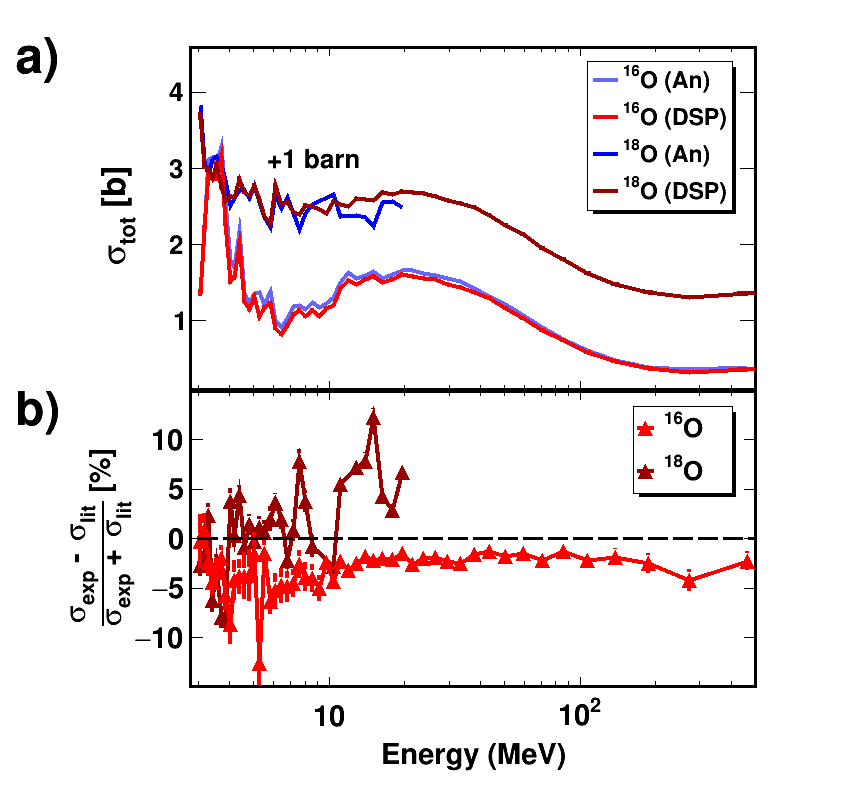
\includegraphics[scale=0.35]{figures/TwoPanelO.png}
    \caption[Neutron \tot\ for \oSixEight: our results and literature data]
    {Neutron \tot\ for \oSixEight: our results and literature data.
        (a) shows our digitizer-measured isotopic results (in shades of red) and
        corresponding analog-measured literature data \cite{Finlay1993, Perey1972, Vaughn1965,
        Salisbury1965} (in shades of blue). The data for \oEight have been
        shifted up by 1 barn, for visibility.
        (b) shows the relative difference between our data
        and literature data that are shown in panel a).
    }
    \label{TwoPanelO}
\end{figure}

\begin{figure}[h]
    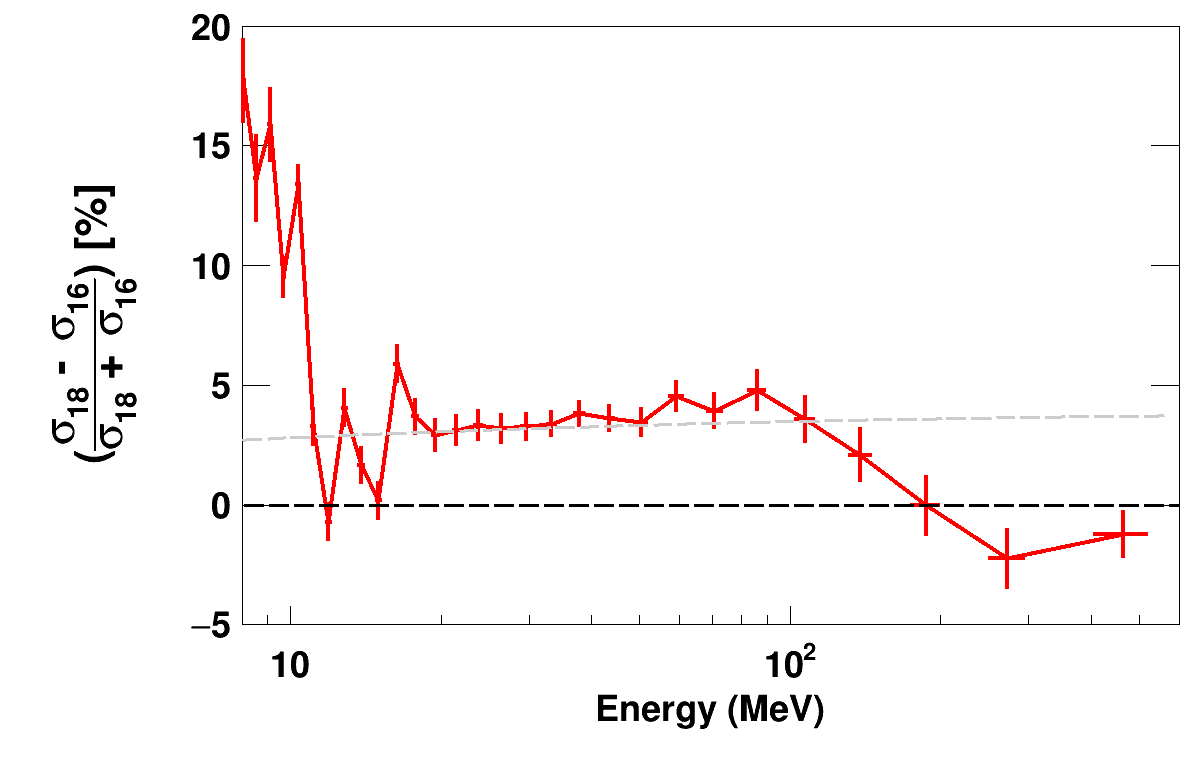
\includegraphics[scale=0.35]{figures/relativeDiff_O18O16.png}
    \caption[\oSixEight\ neutron \tot\ relative difference]
    {\oSixEight\ neutron \tot\ relative difference, from our newly-measured
        data sets (in red). Assuming a simple A$^{\frac{1}{3}}$ size scaling for the
        nuclear radius of \oEight from \oSix, the simple oscillatory model of
        Eq. \ref{OscillatoryModel} prediction for the \oSixEight neutron \tot\ relative
        difference is shown (gray dashed line). From 10-100 MeV, the oscillatory
        model is surprisingly successful at reproducing the relative difference,
        though it fails above 100 MeV as the \oEight neutron \tot\ drops below
    that of \oSix.}
    \label{IsotopicDifferenceO}
\end{figure}

Above 5 MeV, our \oSix\ \tot\ results are within 5\% of those from \cite{Finlay1993}, where
ZnO and BeO were used rather than H$_{2}$O. Below 5 MeV, the rapidly-rising
(n,p) cross section and resonance structure of Zn, Be, and \oSix\ contribute to
increased relative differences. Our measurement on \oEight\ extends the known
neutron \tot\ by over an order of magnitude and shows reasonable agreement to
the previous measurements taken over 50 years ago by \cite{Vaughn1965,Salisbury1965}.
Above 200 MeV, the \oEight\ \tot\ is smaller than the \oSix\ \tot\, a
consequence of the larger neutron elastic phase shift in \oEight\ compared to
\oSix, which pushes the \tot\ minimum to higher energies in \oEight.

\subsection{\niEightFour\ \tot\ results}
\begin{figure}[h]
    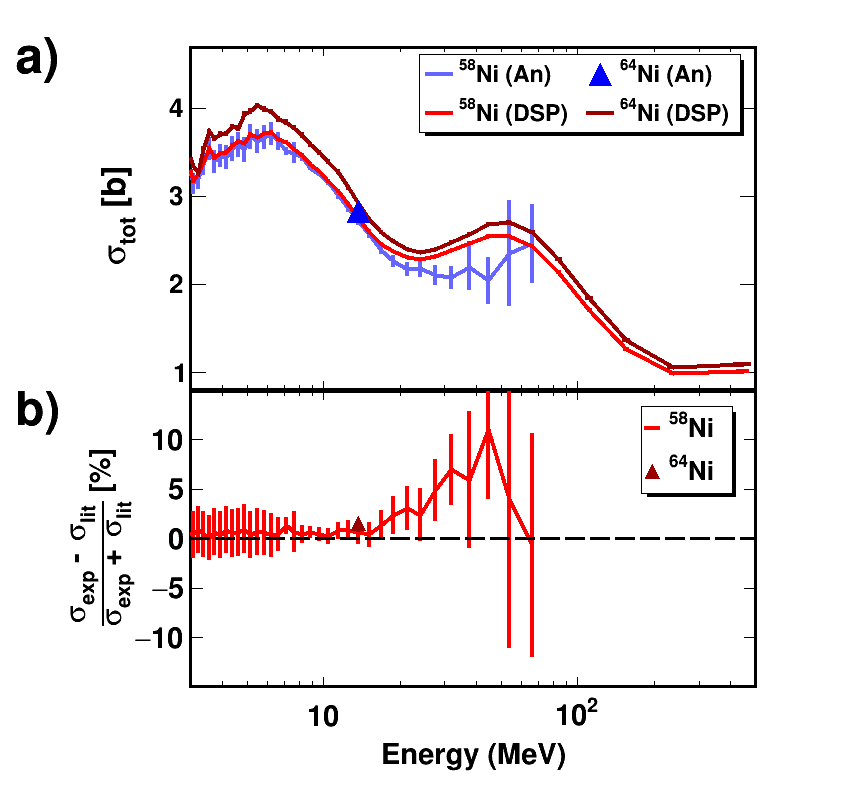
\includegraphics[scale=0.35]{figures/TwoPanelNi.png}
    \caption[Neutron \tot\ for \niEightFour: our results and literature data]
    {
        Neutron \tot\ for \niEightFour: our results and literature data.
        (a) shows our digitizer-measured isotopic results (in shades of red) and
        corresponding analog-measured literature data \cite{Perey1993,
        Dukarevich1967} (in shades of blue). (b) shows the relative difference
        between our data and literature data that are shown in panel a).
    }
    \label{TwoPanelNi}
\end{figure}

\begin{figure}[h]
    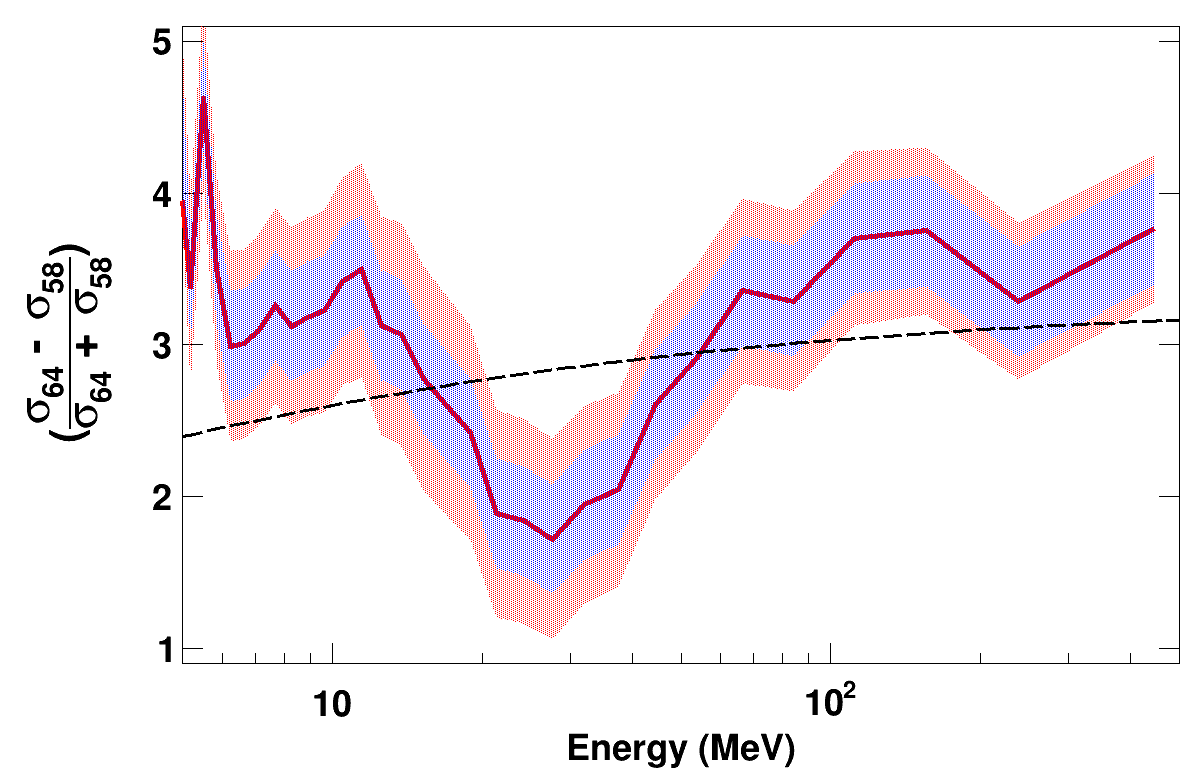
\includegraphics[scale=0.35]{figures/relativeDiff_Ni64Ni58.png}
    \caption[\niEightFour\ neutron \tot\ relative difference]
    {
        \niEightFour\ neutron \tot\ relative difference, from our newly-measured
        data sets (in red). Total error (including statistical and systematic)
        is indicated by the red dotted region. Systematic error only (due to
        uncertainty in the sample areal density) is shown by the blue dotted region.   
        Assuming a simple A$^{\frac{1}{3}}$ size scaling for the
        nuclear radius of \niFour\ from \niEight, the simple oscillatory model of
        Eq. \ref{OscillatoryModel} prediction for the \niEightFour\ neutron \tot\ relative
        difference is shown (black dashed line).
    }
    \label{IsotopicDifferenceNi}
\end{figure}

In contrast to the case of O, no isotopic Ni data was available at all above 100
MeV, and high-precision literature data was only available up to 15 MeV for
\niEight\ \cite{Perey1993} and at only one energy point, 14.2 MeV, for \niFour\
\cite{Dukarevich1967}. Our results extended the energy range to 400 MeV and are
in good agreement with the previous results when their errors are included.

\subsection{\rhThree\ \tot\ results}
\begin{figure}[h]
    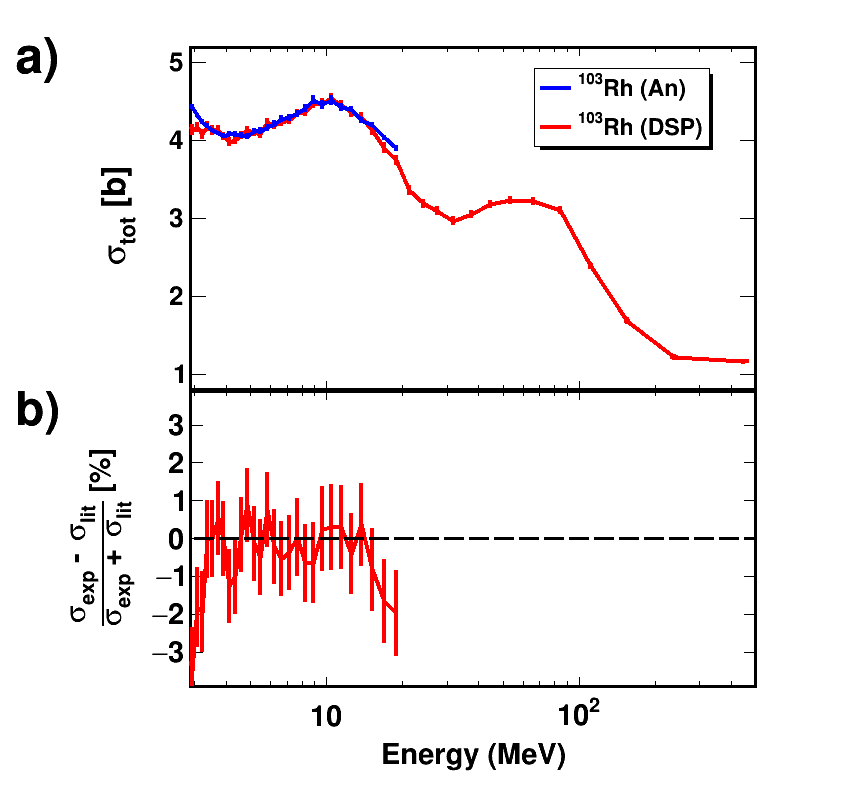
\includegraphics[scale=0.35]{figures/TwoPanelRh.png}
    \caption[Neutron \tot\ for \rhThree: our results and literature data]
    {
        Neutron \tot\ for \rhThree: our results and literature data.
        (a) shows our digitizer-measured isotopic results (in red) and
        corresponding analog-measured literature data \cite{Poenitz1983} (in blue).
        (b) shows the relative difference
        between our data and literature data that are shown in panel a).
    }
    \label{TwoPanelRh}
\end{figure}

The extremely small areal density and the reduced beam
time allotted for our \rhThree\ sample made acquiring sufficient statistics difficult.
Nevertheless, by reducing the energy range and number of bins slightly, we were
able to achieve 1\% statistics for all bins and our results agree with those of
\cite{Poenitz1983} up to 20 MeV. Our results extend the known energy range by over an order of
magnitude up to 400 MeV.

\subsection{\snTwelveFour\ \tot\ results}
\begin{figure}[h]
    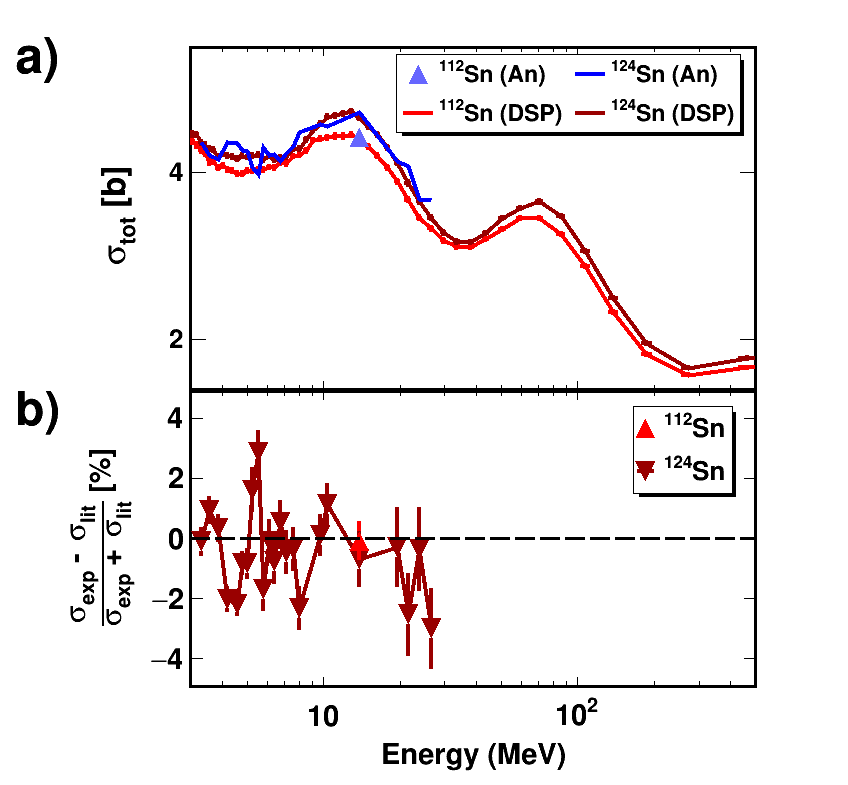
\includegraphics[scale=0.35]{figures/TwoPanelSn.png}
    \caption[Neutron \tot\ for \snTwelveFour: our results and literature data]
    {
        Neutron \tot\ for \snTwelveFour: our results and literature data.
        (a) shows our digitizer-measured isotopic results (in red) and
        corresponding analog-measured literature data \cite{Harper1982, Timokhov1989, 
        Rapaport1980, Dukarevich1967} (in shades of blue).
        (b) shows the relative difference between our data
        and literature data that are shown in panel a). The data sets are in
        excellent agreement where literature data exist, up to 20 MeV.
    }
    \label{TwoPanelSn}
\end{figure}

\begin{figure}[h]
    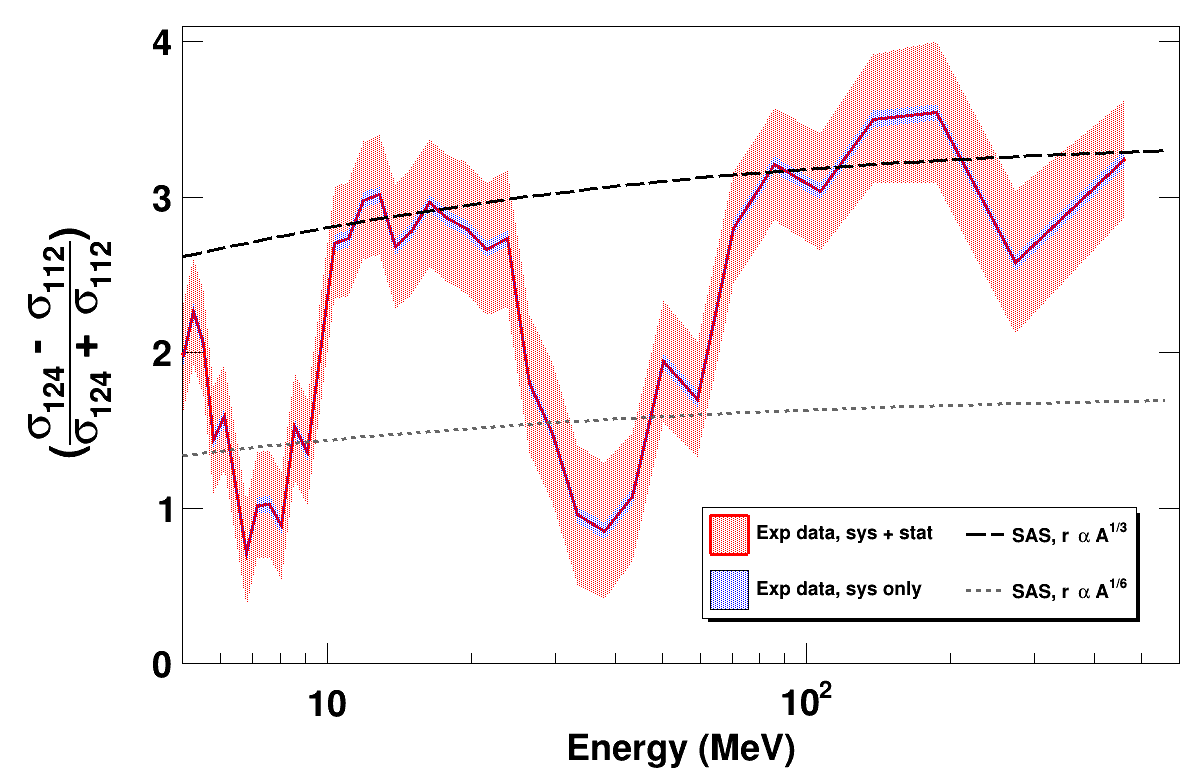
\includegraphics[scale=0.35]{figures/relativeDiff_Sn124Sn112.png}
    \caption[\snTwelveFour\ neutron \tot\ relative difference]
    {
        \snTwelveFour\ neutron \tot\ relative difference, from our newly-measured
        data sets (in red). Total error (including statistical and systematic)
        is indicated by the red dotted region. Systematic error only (due to
        uncertainty in the sample areal density) is shown by the blue dotted region.   
        Assuming a simple A$^{\frac{1}{3}}$ size scaling for the
        nuclear radius of \snFour\ from \snTwelve, the simple oscillatory model of
        Eq. \ref{OscillatoryModel} prediction for the \snTwelveFour\ neutron \tot\ relative
        difference is shown (gray dashed line).
    }
    \label{IsotopicDifferenceSn}
\end{figure}

Similar to Ni isotopes, the only existing Sn isotope neutron \tot\ data was at
low energies, up to 20 MeV for both \snTwelve\ and \snFour\ \cite{Harper1982, Timokhov1989, 
Rapaport1980, Dukarevich1967}. Our results extended the energy range to 400 MeV and are
in excellent agreement, $\approx$1\% difference, with the previous results.

\afterpage{\clearpage}
